\xchapter{Introdução}{}

\acresetall 


Este capítulo apresenta o contexto em que a presente investigação se insere, enfatizando: a apresentação; o problema; os objetivos; as questões de pesquisa; a metodologia; os resultados esperados e como o trabalho está estruturado.

\section{Apresentação}\label{sec:apresentacao}
Desenvolver software não é uma tarefa simples e envolve diversas condicionais, tais como: escopo, prazo e recursos disponíveis. Nesse processo, um problema que pode ocorrer é entregar algo diferente do que era esperado pelo cliente. Isso acontece na maioria das vezes porque as atividades de desenvolvimento dependem da capacidade de interpretação e execução das pessoas que as constroem. Para que esses erros não perdurem e para que se possa identificá-los antes de liberar o software para utilização, existe uma série de atividades, coletivamente chamadas de Validação, Verificação e Teste \cite{DELAMARO2007}. 

\ac{VV} permite que se determine sistematicamente se os requisitos de um sistema estão sendo corretamente tratados e implementados. Por sua vez, a atividade de testes tem por objetivo descobrir defeitos no software, considerando aspectos estruturais e lógicos. Verificar, validar e testar software auxiliam na Garantia de Qualidade do mesmo. Garantia de Qualidade, do termo comumente utilizado (em inglês) \ac{QA}, é o processo geral de definição de como a qualidade de software pode ser alcançada, e como a empresas que trabalham com desenvolvimento sabe que o software tem o nível de qualidade necessário. \ac{QA} estabelece processos, procedimentos e padrões que conduzem a um software de qualidade \cite{HIRAMA2011}. 

O presente trabalho tem como foco a atividade de teste. Os testes são normalmente executados e reportados durante as etapas de desenvolvimento do software. Espera-se que haja uma grande massa de testes realizada antes de se disponibilizar uma versão estável do software. Entretanto, existe uma técnica de testes, denominada \textbf{teste de regressão}, que deve ser considerada quando é necessário realizar a manutenção do software, quer perfectiva, corretiva, adaptativa ou preventiva \cite{DBLP:series/springer/Mens08}. O teste de regressão tem como objetivo fornecer confiança de que as alterações recém-introduzidas não compromete o comportamento funcional da parte existente e inalterada do software \cite{Yoo:2012:RTM:2284811.2284813}.

No teste de regressão, uma das possíveis abordagens é a reexecução de todos os casos de testes da versão original do software. Porém, esse procedimento tende a gerar um grande esforço da equipe de testes, a depender da quantidade de casos de teste. A literatura apresenta uma série de técnicas para lidar com este problema, em particular no sentido de propor mecanismos para reduzir o número de reexecuções de casos de testes, sem perder a cobertura do código fonte e a capacidade de detecção de defeitos  \cite{Graves:2001:ESR:367008.367020,ENGSTROM201014,KAZMI2017,ROMANO201862}.

Segundo \citeonline{Yoo:2012:RTM:2284811.2284813} as técnicas de Teste de Regressão são classificadas como: Técnicas de Seleção; Técnicas de Minimização; e Técnicas de Priorização. As técnicas de seleção, buscam reduzir a quantidade de casos de testes a serem reexecutados selecionando-os de acordo com a parte do software que foi alterada. As técnicas de minimização, propõe a remoção de casos de testes redundantes. E, as técnicas de priorização tem como foco encontrar o conjunto mais representativo de casos de testes a serem reexecutados.

Dentre os domínios de aplicação emergentes, testes de regressão apresentam-se como uma estratégia viável para lidar com a complexidade - e a constante evolução - dos \ac{APPS}, tais como: experiência do usuário, portabilidade, segurança, conectividade e desempenho. Neste cenário, o presente trabalho tem como foco a análise da evolução das técnicas de seleção de teste de regressão no desenvolvimento de \ac{APPS} para Android.


\section{Problema}\label{sec:problema}

Os dispositivos móveis tem sido cada vez mais utilizados no cotidiano, em alguns casos com maior parcela de mercado do que os tradicionais Desktop \cite{Do2016RedroidAR}. Pesquisas de mercado recentes, considerando o período entre os meses de agosto de 2019 a agosto de 2020, indicam que o \textbf{Android} é o sistema operacional mais popular para os dispositivos móveis, com 74.25\% dos usuários \footnote{\url{http://gs.statcounter.com/os-market-share/mobile/worldwide}}.

\begin{figure}[!htb]
\centering
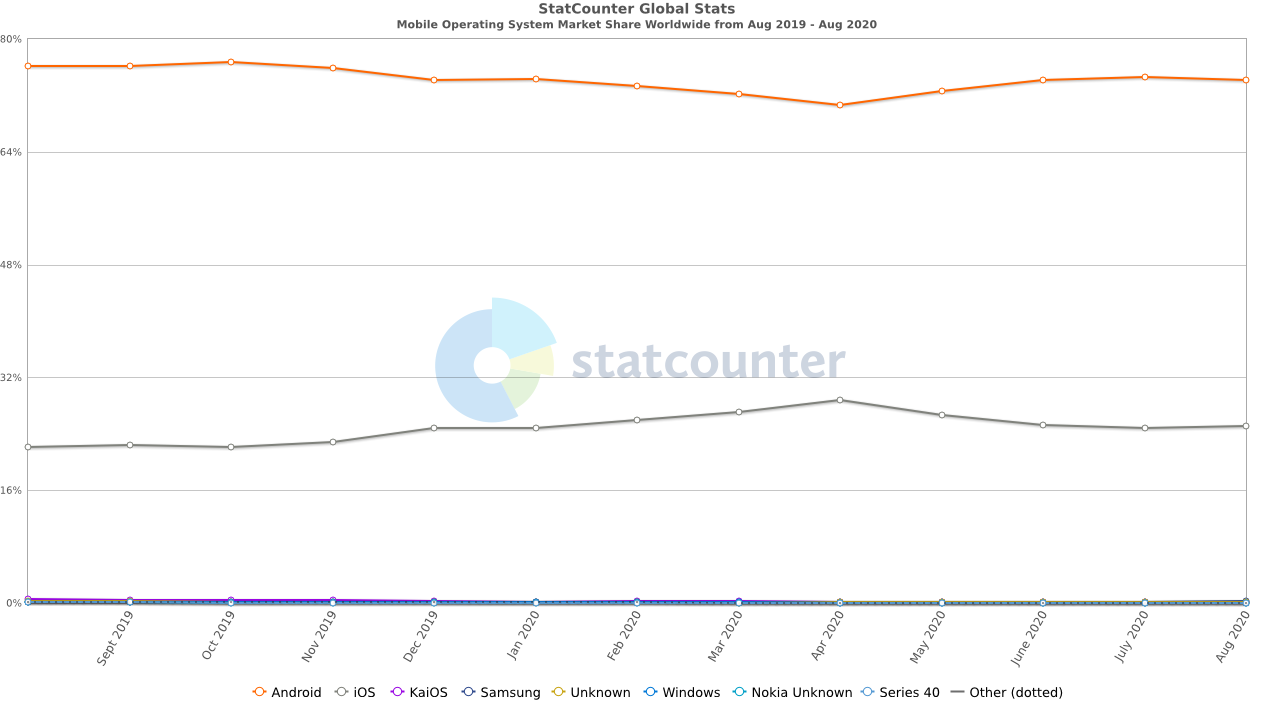
\includegraphics[width=.8\textwidth]{images/usuariosAndroid.png}
\caption{\textit{Distribuição mundial do uso de sistemas operacionais para \ac{APPS}.}}
\label{figure:usuariosAndroid}
\end{figure}


Segundo \citeonline{Do2016RedroidAR}, a plataforma móvel está se separando de uma variedade de áreas de aplicativos de Desktop, tais como entretenimento, comércio eletrônico e mídia social. Assim, os desenvolvedores são obrigados a produzir \ac{APPS} de alta qualidade, em particular no que diz respeito a requisitos não-funcionais como portabilidade, confiabilidade e segurança.


Nos últimos anos, uma grande quantidade de pesquisas tem sido realizadas para prover uma maior confiabilidade dos \ac{APPS}, por exemplo, aplicando testes automatizados \cite{7927972, 8424973, 8453877}. No entanto, a maioria das pesquisas está focada no teste de uma versão única de aplicativos móveis \cite{Do2016RedroidAR}. Em virtude da constante evolução dos aplicativos e a necessidade de avaliar se as alterações realizadas não afetaram seu comportamento funcional, os testes de regressão se apresentam como uma estratégia viável\cite{8377661} na detecção de defeitos.   


%Como os \ac{APPS} evoluem com frequência, é importante que os desenvolvedores façam uso de técnicas de teste de regressão, dado seu potencial em identificar problemas no código decorrentes de mudanças no software \cite{8377661}.%

Ao tratar de técnicas de teste de regressão, a literatura apresenta diversos trabalhos que fazem uso de técnicas tradicionais, i.e., concebidas para testar sistemas Desktop \cite{536955}, \cite{ENGSTROM201014}. Entretanto, embora muitas abordagens eficientes e eficazes tenham sido propostas, há pouca evidência sobre a aplicação direta dessas técnicas para o teste de \ac{APPS} \cite{Do2016RedroidAR}. %Um importante fator que causa a incompatibilidade é a diferença entre a arquitetura do sistema da plataforma móvel e a plataforma Desktop.%

%Segundo \citeonline{5954416}, a qualidade dos \ac{APPS} é geralmente ruim. Um dos fatores da falta de qualidade são processos de desenvolvimento muito rápidos em que a atividade de teste é negligenciada ou conduzida de forma superficial, uma vez que é considerada demasiado complexa, difícil de automatizar, dispendiosa e demorada.% 

Em virtude do crescimento do mercado de dispositivos móveis e da necessidade de produzir \ac{APPS} com qualidade, pesquisas recentes tem apresentado o desenvolvimento de técnicas implementadas por ferramentas de teste de regressão voltadas para aplicações em Android \cite{Do2016RedroidAR}, \cite{Choi:2018:DMA:3180155.3180173}, \cite{8377661}, \cite{5954416}, \cite{7927972}, \cite{8424973}, \cite{6339502}, \cite{6569773}, \cite{7427895}, \cite{7832883}, \cite{7833000}. Alguns desses estudos tratam de experimentos que apresentam evidências empíricas acerca da eficiência/eficácia da ferramenta proposta neste cenário. %Alguns desses estudos tratam de experimentos com comprovação empírica para comprovar a eficiência/eficácia da ferramenta proposta neste cenário.%

%Embora a literatura tenha dedicado esforços em produzir evidências sobre a criação de novas técnicas de teste de regressão para Android, os estudos existentes são bastante limitados no que diz respeito a demonstrar evidências empíricas que garantam quais são as técnicas de seleção de teste de regressão implementadas por ferramentas mais aplicáveis no desenvolvimento de \ac{APPS} Android, e também, como estas técnicas são aplicadas por profissionais da indústria de \ac{APPS}. Neste sentido, é fundamental que novas pesquisas sejam desenvolvidas, de modo a ampliar o conjunto de evidências sobre essa aplicabilidade.%

Embora a literatura tenha dedicado esforços na apresentação de evidências empíricas acerca das técnicas de teste de regressão aplicadas a projetos Android, os estudos existentes são bastante limitados no que diz respeito a prover evidências empíricas sobre quais são as técnicas de seleção de teste de regressão implementadas por ferramentas mais aplicáveis no desenvolvimento de \ac{APPS} Android, e também, como estas técnicas são utilizadas por profissionais da indústria de \ac{APPS}. Neste sentido, é fundamental que novas pesquisas sejam desenvolvidas, de modo a ampliar o conjunto de evidências sobre essa aplicabilidade.

Dado a complexidade do problema ora descrito, este estudo buscará responder à seguinte questão de pesquisa principal:
\leavevspace 

\begin{center}
    \noindent\fbox{ 
        \parbox{.8\textwidth}
        {
        \begin{center}
            
            \textbf{Quais são as técnicas de seleção de teste de regressão implementadas por ferramentas adequadas para projetos de \ac{APPS} Android?}
        \end{center}
        }
    }
\end{center}

\vspace{.5em}

Esta questão foi refinada em questões específicas:
\vspace{.5em}

\begin{enumerate}[label=\bf QP\arabic*,leftmargin=1.8cm]
    
    \item \textbf{Quais são as técnicas de seleção de teste de regressão apresentadas na literatura?} Essa questão de pesquisa tem como objetivo levantar quais são as técnicas de seleção de teste de regressão disponíveis na literatura, e quais destas, se aplicam ao desenvolvimento de \ac{APPS} para Android.
    %Essa questão de pesquisa será respondida com a revisão estruturada da literatura sobre Técnicas de Seleção de Teste de Regressão.%
    
    \item \textbf{Existem ferramentas de teste de regressão aplicadas a \ac{APPS} Android disponíveis para utilização (open source ou proprietárias) implementadas a partir de técnicas de seleção de teste de regressão?} Essa questão de pesquisa tem como objetivo identificar se existem ferramentas implementadas a partir do estudo das técnicas de seleção de teste de regressão que estejam disponíveis para utilização por profissionais/pesquisadores da    área.
    
    %Essa questão de pesquisa será respondida com a revisão estruturada da literatura sobre ferramentas de teste de regressão.%
    
    \item \textbf{Qual a aplicabilidade das técnicas de seleção de teste de regressão na indústria de \ac{APPS} para Android?} Essa questão de pesquisa tem como objetivo identificar se as técnicas de seleção de teste de regressão encontradas na literatura são utilizadas por profissionais/pesquisadores que atuam em projetos de \ac{APPS} para Android.
    
    
    %{Qual a perspectiva de acadêmicos e profissionais sobre a aplicação das técnicas de seleção de teste de regressão implementadas por ferramentas em projetos de \ac{APPS} Android?}Essa questão de pesquisa será respondida com a aplicação de um \textit{Survey} e de realização de Entrevistas com estudantes/profissionais que atuam em projetos de apps Android.%

\end{enumerate}



\subsection{Objetivos}

Compreendendo que o estudo das técnicas de seleção de teste de regressão para Android é um campo em expansão, o presente trabalho tem como objetivo \textbf{realizar uma avaliação empírica das técnicas de seleção de teste de regressão implementadas por ferramentas aplicadas a \ac{APPS} Android}.

Os seguintes objetivos específicos foram definidos para esta investigação:

\begin{enumerate}[label=\bf O\arabic*,leftmargin=1.5cm]

    \item \textbf{Levantar quais são as técnicas de seleção de teste de regressão que a literatura apresenta.} Para alcançar esse objetivo, será realizado uma revisão estruturada de literatura sobre técnicas de seleção de teste de regressão.
    
    \item \textbf{Verificar quais são as ferramentas de teste de regressão aplicadas a \ac{APPS} Android disponíveis para uso (open source ou proprietárias), e se as mesmas foram implementadas baseadas nas técnicas de seleção de teste de regressão.} Para alcançar esse objetivo, será realizado uma revisão estruturada de literatura sobre ferramentas de teste de regressão.
    
    \item \textbf{Identificar como é realizado o processo de teste de regressão por profissionais/pesquisadores que atuam em projetos de desenvolvimento de \ac{APPS} para Android.} Para alcançar esse objetivo, será aplicado um \textit{Survey} e realizado entrevistas com profissionais/pesquisadores que trabalham com projetos de \ac{APPS} para Android.


\end{enumerate}



\section{Metodologia}\label{sec:metodologia}


Esta Seção apresenta a metodologia utilizada para desenvolver este trabalho e alcançar os objetivos propostos:


\begin{itemize}
  \item \textbf{Fase 1}: Etapa conceitual que tem como objetivo tratar dos conhecimentos referentes ao tema proposto.
  
  Esta etapa visa levantar a bibliografia das áreas sob investigação, para compreender conceitos fundamentais. São elas: evolução de software; qualidade de software; testes de software; teste de regressão; técnicas de seleção; estratégias de testes de aplicações para dispositivos móveis; ferramentas para teste de \ac{APPS} Android.
  
  O levantamento bibliográfico foi feito de forma estruturada, com a leitura de livros e artigos sobre os tópicos abordados na pesquisa. Inicialmente uma leitura mais ampla em busca de um conhecimento inicial, e em uma segunda fase, com leituras específicas de textos com relação direta a este trabalho, utilizando a metodologia de mapeamento sistemático proposto por \citeonline{Wohlin:2012:ESE:2349018}.
  
  \item \textbf{Fase 2}: Refere-se ao Survey.
  
  Esta etapa contempla a aplicação de um \textit{Survey} para profissionais/pesquisadores que trabalham em projetos de \ac{APPS} para Android.
  
  Com o objetivo de compreender como testadores e desenvolvedores, realizam o teste de regressão em projetos de apps para Android, utilizando a metodologia proposta por Kasunic \citeonline{Kasunic2005DesigningAE} e aplicando os princípios de pesquisa definidos por Kitchenham et al. \citeonline{Kitchenham:2002:PSR:566493.566495}, realizamos um \textit{Survey} com 100 profissionais/pesquisadores que atuam em projetos de \ac{APPS} para Android. 
  
  Os resultados preliminares demostraram que o processo de teste de \ac{APPS} para Android é feito majoritariamente de forma manual e sem suporte de ferramentas, bem como, identificamos que apenas 51\% dos respondentes realizam teste de regressão.
 
  \item \textbf{Fase 3:} Refere-se as Entrevistas.
  
  %Esta etapa refere-se a realização de entrevistas com uma amostra de profissionais que trabalham no processo de testes de \ac{APPS} Android e possuem experiência na área, para compreender questões específicas referente a este processo.%
  Esta etapa refere-se a realização de entrevistas com profissionais que trabalham em projetos de \ac{APPS} para Android e possuem experiência na área de testes de apps. Queremos complementar os resultados obtidos com o \textit{Survey}, explorando questões não abordadas na etapa anterior, tais como, identificar quais \textit{features} das ferramentas de teste para \ac{APPS} Android atendem os profissionais/pesquisadores da área, e quais features precisam ser implementadas. Bem como, compreender como o teste de regressão é executado. Utilizaremos o design de entrevistas semi-estruturadas elencado em \citeoline{HOVE:2005}.
  
  \item \textbf{Fase 4}:\textit{Evidences Briefings}
  
  Esta etapa refere-se na confecção de \textit{Evidences Briefings} para reportar a pesquisadores e profissionais, os achados referente a são realizados os testes de regressão, por profissionais e pesquisadores, que atuam em projetos de apps para Android. Utilizaremos a metodologia analisada em \citeonline{CARTAXO:2016}.
  
\end{itemize}

\section{Resultados Esperados}\label{sec:resultadosesperados}

%Ao final deste trabalho, espera-se contribuir com os seguintes resultados:

Com o desenvolvimento do presente estudo, espera-se contribuir com o estado da arte na área de qualidade de software, em particular no que diz respeito ao uso de técnicas de seleção de teste de regressão para o desenvolvimento de projetos de \ac{APPS} para Android. A seguir, sintetizamos as principais contribuições esperadas: 


\begin{itemize}

    \item Contribuir com o corpo de conhecimento sobre o uso de técnicas de seleção para o desenvolvimento de \ac{APPS} para Android, com base na síntese de evidências disponíveis na literatura.
    
    \item Coletar e analisar dados, no sentido de prover evidências empíricas sobre quais as técnicas de seleção implementadas por ferramentas são mais adequadas para projetos de \ac{APPS} Android.
    
    \item Identificar a aplicabilidade das técnicas de seleção de teste de regressão por profissionais/pesquisadores que trabalham no desenvolvimento de projetos de \ac{APPS} para Android.
    
    \item Apresentar o potencial, em termos de \textit{features} implementadas, das ferramentas de teste de regressão disponíveis para projetos Android, e levantar oportunidades para implementações futuras.

\end{itemize}


\section{Estrutura do Trabalho}\label{sec:estruturadotrabalho}

Os demais capítulos desta qualificação estão estruturados como segue: 
\begin{itemize}
\item \textbf{Capítulo 2}: Fundamentação Teórico, Conceitos e Aplicabilidades;
\item \textbf{Capítulo 3}: \textit{Survey};
\item \textbf{Capítulo 4}: Trabalhos Relacionados e Cronograma de Atividades.
\end{itemize}